% {{{ Preamble ----------------------------------------------------------------
\documentclass{beamer}

% encodings, fonts etc.
\usepackage[utf8x]{inputenc}
\usepackage[T1]{fontenc}

% Hold kæft utf
\makeatletter
\def\UTFviii@defined#1{%
  \ifx#1\relax
      ?%
  \else\expandafter
    #1%
  \fi
}

\makeatother

% math packages
\usepackage{amsmath, amssymb, amsthm}
\usepackage{mathtools}

% beamer configuration
\usetheme{Copenhagen}
%\usetheme{metropolis}
\beamertemplatenavigationsymbolsempty
%\setbeamertemplate{theorems}[numbered]
\setbeamersize{description width=2.0em}

%\usepackage{pgfpages}
%\setbeameroption{show notes}
%\setbeameroption{show notes on second screen=right}

% algorithms
\usepackage{algorithm}
\usepackage[noend]{algpseudocode}

% misc. packages
\usepackage{float}
\usepackage{varwidth}
\usepackage{listings}
\lstset{
  %breaklines=true,
  keepspaces=true,
  %frame=ltrb,
  %framesep=1pt,
  %commentstyle=\color{grey},
  basicstyle=\ttfamily\tiny,
  %numbers=left,
  title=\lstname,
  %columns=fullflexible,
  inputencoding=utf8,
  extendedchars=true,
}

% graphics and tikz
\usepackage{pgf}
\usepackage{tikz}
\usetikzlibrary{positioning,arrows,calc}
\tikzset{
    on grid,
    node distance=3cm,
    auto,
    block/.style = {
        draw,
        shape=rectangle,
        minimum height=3em,
        minimum width=3em,
        line width=1pt
    },
    empty/.style = {
        shape=rectangle,
        minimum height=3em,
        minimum width=3em
    },
    >=latex',
}


% mathematics
\newtheorem{proposition}{Proposition}

\renewcommand{\tt}{\texttt}

% title page
\title{Basic logic circuits}
\author[Carl-Johannes Johnsen]{
  \mbox{Carl-Johannes Johnsen}}
\institute{Department of Computer Science\\
           University of Copenhagen}
%\date{December 22, 2016}
% }}} -------------------------------------------------------------------------

\begin{document}

% {{{ Title page --------------------------------------------------------------
\frame{\titlepage}
% }}} -------------------------------------------------------------------------

% {{{ Table of contents -------------------------------------------------------
%\begin{frame}
%  \frametitle{Outline}
%  \tableofcontents
%\end{frame}
% }}} -------------------------------------------------------------------------

\section{Introduction}
\begin{frame}
    In this lecture, we will be looking at some basic combinatorial circuits,
    and how to implement them using SME.

    \vspace{\baselineskip}
    We will try to construct the following circuits:
    \begin{itemize}
        \item Basic logical gates
        \item Decoder
        \item Half adder
        \item Full adder
        \item $n$-bit adder
    \end{itemize}
\end{frame}

\section{Basic logic gates}
\subsection{Theory}
\begin{frame}
    A logic gate is a circuit abstraction with one or more inputs, and an
    output. It computes its output value based on the logic function it is
    mimicing. We look at the four basic logic gates:
    \begin{description}
        \item[\tt{AND}] - outputs \tt{1} iff. all of its inputs are \tt{1},
            otherwise \tt{0}
        \item[\tt{OR}] - outputs \tt{1} if one or more of its inputs are
            \tt{1}, otherwise \tt{0}
        \item[\tt{NOT}] - outputs the inverse of its input, e.g. \tt{1} becomes
            \tt{0}
        \item[\tt{XOR}] - outputs \tt{1} iff. exactly one of its inputs are
            \tt{1}, otherwise \tt{0}
    \end{description}
\end{frame}
\begin{frame}
    \begin{center}
        \begin{tabular}{cc|cccc}
            \hline
            \tt{Bit1} & \tt{Bit2} & \tt{AND} & \tt{OR} & \tt{NOT} & \tt{XOR} \\
            \hline
            \tt{0} & \tt{0} & \tt{0} & \tt{0} & \tt{1} & \tt{0} \\
            \tt{0} & \tt{1} & \tt{0} & \tt{1} & \tt{1} & \tt{1} \\
            \tt{1} & \tt{0} & \tt{0} & \tt{1} & \tt{0} & \tt{1} \\
            \tt{1} & \tt{1} & \tt{1} & \tt{1} & \tt{0} & \tt{0} \\
            \hline
        \end{tabular}
    \end{center}
\end{frame}

\subsection{Implementation}
\begin{frame}
    Implementing each of the gates in SME is very simple. As with CSP, we
    create a process for each gate. Each gate has two input busses, except for
    \tt{NOT}, which only has one, and one output bus. Each bus contains one
    \tt{bool} value. We choose \tt{bool}, to ensure that the later VHDL
    generation will construct wires, and not full-blown 32-bit busses.

    \vspace{\baselineskip}
    Each of the processes will take its inputs, and put the result of its logic
    function on its output bus.
\end{frame}
\begin{frame}[fragile]
    \lstinputlisting[firstline=2,title=Buses]{../../sme/src/Examples/LogicGates/Buses.cs}
    Note: for compactability, the inputs and outputs have been gathered on a
    single bus.
\end{frame}
\begin{frame}[fragile]
    \lstinputlisting[firstline=8,lastline=20,title=AND gate]{../../sme/src/Examples/LogicGates/Gates.cs}
\end{frame}

\subsection{Testing}
\begin{frame}
    To test our implementation, we are going to need a process, which is going
    to send data on the input bus for each of the components, and is going to
    verify that each component outputs the expected value. Since we are only
    working with two bits, we can try all the possible combination of inputs.
\end{frame}
\begin{frame}
    \begin{figure}
        \centering
        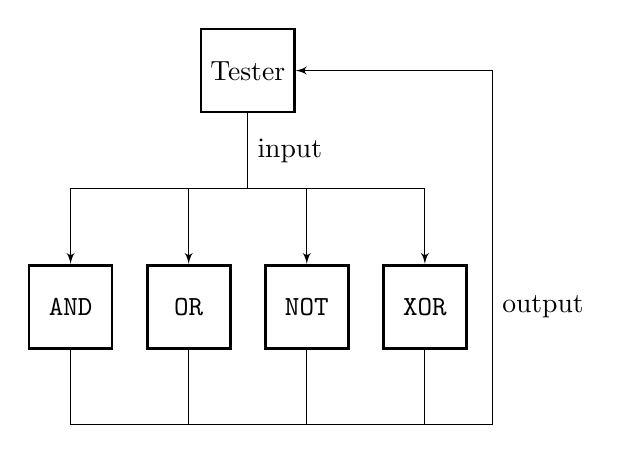
\begin{tikzpicture}[node distance=1.5cm]
            \node[block] (and) {\texttt{AND}};
            \node[block, right of=and] (or) {\texttt{OR}};
            \node[block, right of=or] (not) {\texttt{NOT}};
            \node[block, right of=not] (xor) {\texttt{XOR}};
            \node[above of=and] (input) at ($(or)!0.5!(not)$) {};
            \node[block, above of=input] (tester) {Tester};

            \path[-] (tester) edge node[midway, right] {input} (input.center);
            \path[draw, ->] (input.center) -| (and.north);
            \path[draw, ->] (input.center) -| (or.north);
            \path[draw, ->] (input.center) -| (not.north);
            \path[draw, ->] (input.center) -| (xor.north);

            \node[below of=and] (output) at ($(or)!0.5!(not)$) {};
            \node[right of=xor] (a) {output};

            \path[draw, -] (and.south) |- (output.center);
            \path[draw, -] (or.south) |- (output.center);
            \path[draw, -] (not.south) |- (output.center);
            \path[draw, -] (xor.south) |- (output.center);

            \path[draw, -] (output.center) -| (a.west);
            \path[draw, ->] (a.west) |- (tester.east);
        \end{tikzpicture}
        \label{fig:logic-test}
    \end{figure}
\end{frame}

\section{Decoder}
\subsection{Theory}
\begin{frame}
    Now that we have made some basic gates, we are going to construct our first
    combinatorial circuit: The decoder.

    \vspace{\baselineskip}
    A decoder takes an $n$-bit input, and produces an $2^n$-bit output, where
    the $n$th output bit is set to \tt{1}, if the input is the binary
    representation of $n$. All the other output bits are set to \tt{0}.
\end{frame}

\subsection{Implementation}
\begin{frame}
    We will start by looking at a 2-bit decoder for simplicity. To implement
    the decoder, we will combine the basic logic gates as follows:

    \vspace{\baselineskip}
    \begin{figure}
        \centering
        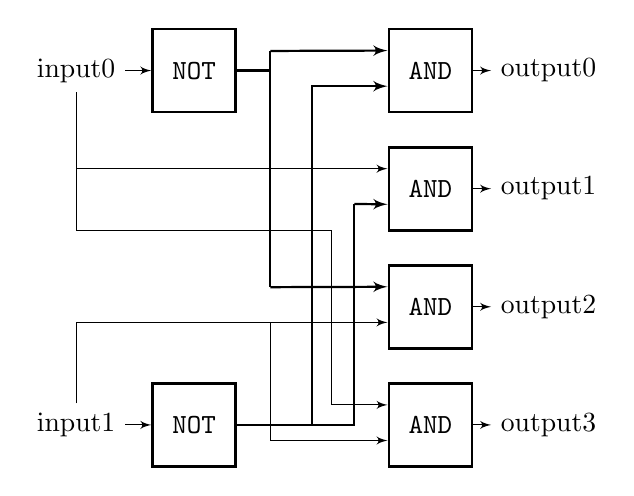
\begin{tikzpicture}[node distance=1.5cm]
            \node[block] (and0) {\texttt{AND}};
            \node[block, below of=and0] (and1) {\texttt{AND}};
            \node[block, below of=and1] (and2) {\texttt{AND}};
            \node[block, below of=and2] (and3) {\texttt{AND}};

            \node[right of=and0] (output0) {output0};
            \node[right of=and1] (output1) {output1};
            \node[right of=and2] (output2) {output2};
            \node[right of=and3] (output3) {output3};

            \path[draw, ->] (and0) -- (output0);
            \path[draw, ->] (and1) -- (output1);
            \path[draw, ->] (and2) -- (output2);
            \path[draw, ->] (and3) -- (output3);

            \node[empty, left of=and0] (andinp0) {};
            \node[empty, left of=and1] (andinp1) {};
            \node[empty, left of=and2] (andinp2) {};
            \node[empty, left of=and3] (andinp3) {};

            \node[block, left of=andinp0] (not0) {\texttt{NOT}};
            \node[block, left of=andinp3] (not1) {\texttt{NOT}};

            \node[left of=not0] (input0) {input0};
            \node[left of=not1] (input1) {input1};

            \path[draw, ->] (input0) -- (not0);
            \path[draw, ->] (input1) -- (not1);

            \path[draw, thick, -] (not0) -| (andinp0.155);
            \path[draw, thick, ->] (andinp0.155) -- (and0.155);
            \path[draw, thick, -] (not1.east) -| (andinp0.south);
            \path[draw, thick, ->] (andinp0.south) |- (and0.200);

            \path[draw, ->] (input0) |- (and1.155);
            \path[draw, thick, -] (not1.east) -| (andinp1.340);
            \path[draw, thick, ->] (andinp1.340) -- (and1.200);

            \path[draw, thick, -] (not0.east) -| (andinp2.155);
            \path[draw, thick, ->] (andinp2.155) -- (and2.155);
            \path[draw, ->] (input1.north) |- (and2.200);

            \path[draw, -] (input0) |- (andinp1.295);
            \path[draw, ->] (andinp1.295) |- (and3.155);
            \path[draw, -] (input1) |- (andinp2.200);
            \path[draw, ->] (andinp2.200) |- (and3.200);

        \end{tikzpicture}
        \label{fig:2-bit-decoder}
    \end{figure}
\end{frame}
\begin{frame}[fragile]
    \lstinputlisting[firstline=2,title=Buses.cs]{../../sme/src/Examples/Decoder/Buses.cs}
\end{frame}
\begin{frame}
    \lstinputlisting[firstline=20,lastline=32,title=Decoder.cs]{../../sme/src/Examples/Decoder/Decoder.cs}
\end{frame}
\begin{frame}
    Now, we also want to construct an $n$-bit decoder, however, this is not
    trivial, as SME requires everything to be known at compile time, and we
    cannot make a generic process, as these depend on the names of the buses.

    \vspace{\baselineskip}
    To solve this problem, we can use C\# templates:
    \begin{itemize}
        \item For each input bit, create a bus
        \item For each bus, create a \tt{NOT} gate
        \item Create $2^n$ output busses
        \item For each output bus, attach an \tt{AND} gate
        \item Connect the input busses and the output from the \tt{NOT} gates,
            so that the binary representation of $n$ will produce a \tt{1} at
            the $n$th \tt{AND} gate
    \end{itemize}
\end{frame}
\begin{frame}[fragile]
    \lstinputlisting[firstline=2,title=Buses.tt]{../../sme/src/Examples/ScalDecoder/Buses.tt}
\end{frame}
\begin{frame}[fragile]
    \lstinputlisting[firstline=23,title=Decoder.tt]{../../sme/src/Examples/ScalDecoder/Decoder.tt}
\end{frame}

\subsection{Testing}
\begin{frame}
    As with the basic logic gates, we need to construct a test process, which
    sends input to the circuit, and verifies that the output is as expected. In
    the case of our 2-bit decoder, we can also try all possible ($2^2=4$)
    values.

    \vspace{\baselineskip}
    To test our $n$-bit decoder we need to construct another template, which
    will try all possible combinations.
\end{frame}

\section{Adder}
\subsection{Theory}
\begin{frame}
    The final circuit we will be looking at is the adder. To construct a full
    $n$-bit adder, we are going to need two subcomponents: An half-adder and an
    full-adder, both of which can be implemented using the basic logic gates.

    \vspace{\baselineskip}
    The half-adder takes two input bits, and produces two output bits. The
    first output bit is the \tt{sum} bit, and the second is the \tt{carry} bit.

    \vspace{\baselineskip}
    The full-adder is similar to the half-adder, with the only difference
    being an additional input.
\end{frame}
\begin{frame}
    The combinatorial circuit for the half-adder.
    \begin{figure}
        \centering
        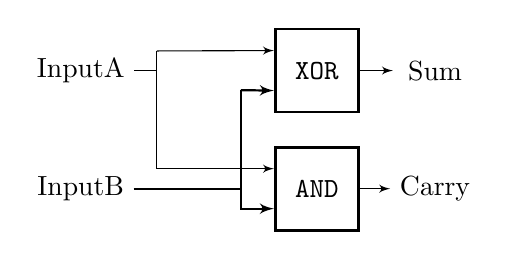
\begin{tikzpicture}[node distance=1.5cm]
            \node[block] (xor) {\texttt{XOR}};
            \node[block, below of=xor] (and) {\texttt{AND}};

            \node[empty, left of=xor] (xorin) {};
            \node[empty, left of=and] (andin) {};

            \node[left of=xorin] (inputa) {InputA};
            \node[left of=andin] (inputb) {InputB};

            \node[empty, right of=xor] (sum) {Sum};
            \node[empty, right of=and] (carry) {Carry};

            \path[draw, -] (inputa) -| (xorin.155);
            \path[draw, ->] (xorin.155) -- (xor.155);
            \path[draw, ->] (xorin.west) |- (and.155);

            \path[draw, thick, -] (inputb.east) -| (xorin.335);
            \path[draw, thick, ->] (xorin.335) -- (xor.205);
            \path[draw, thick, ->] (andin.east) |- (and.205);

            \path[draw, ->] (xor) -- (sum);
            \path[draw, ->] (and) -- (carry);
        \end{tikzpicture}
        \label{fig:half-adder}
    \end{figure}
\end{frame}
\begin{frame}
    The combinatorial circuit for the full-adder.
    \begin{figure}
        \centering
        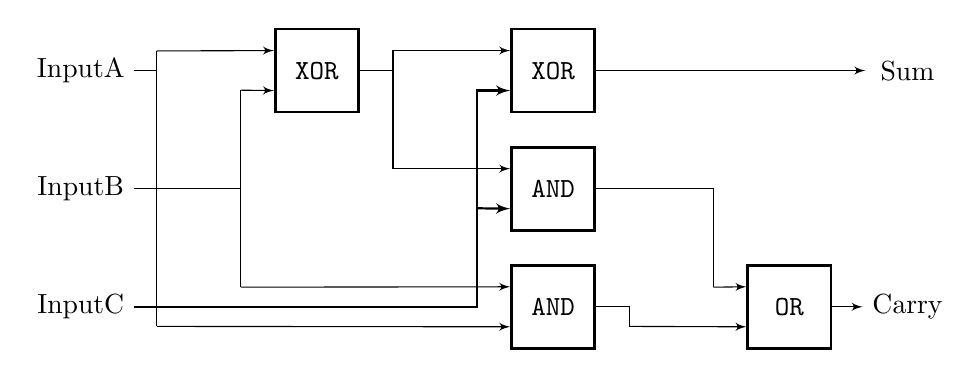
\begin{tikzpicture}[node distance=1.5cm]
            \node[block] (or) {\texttt{OR}};
            \node[empty, left of=or] (orin) {};
            \node[block, left of=orin] (and1) {\texttt{AND}};
            \node[block, above of=and1] (and0) {\texttt{AND}};
            \node[empty, left of=and0] (and0in) {};
            \node[block, above of=and0] (xor1) {\texttt{XOR}};
            \node[empty, left of=xor1] (xor1in) {};
            \node[block, left of=xor1in] (xor0) {\texttt{XOR}};
            \node[empty, left of=xor0] (xor0in) {};
            \node[empty, left of=xor0in] (inputa) {InputA};
            \node[empty, below of=inputa] (inputb) {InputB};
            \node[empty, below of=inputb] (inputc) {InputC};
            \node[empty, right of=inputc] (inputcout) {};
            \node[empty, right of=xor1] (sum) {};
            \node[empty, right of=sum] (summ) {};
            \node[empty, right of=summ] (summm) {Sum};
            \node[empty, right of=or] (carry) {Carry};

            \path[draw, -] (inputa.east) -| (xor0in.155);
            \path[draw, ->] (xor0in.155) -- (xor0.155);
            \path[draw, -] (inputb.east) -| (xor0in.335);
            \path[draw, ->] (xor0in.335) -- (xor0.205);

            \path[draw, -] (inputa.east) -| (inputcout.205);
            \path[draw, ->] (inputcout.205) -- (and1.205);
            \path[draw, -] (inputb.east) -| (inputcout.25);
            \path[draw, ->] (inputcout.25) -- (and1.155);

            \path[draw, thick, -] (inputc.east) -| (and0in.335);
            \path[draw, thick, ->] (and0in.335) -- (and0.205);
            \path[draw, thick, ->] (and0in.335) |- (xor1.205);

            \path[draw, -] (xor0.east) -- (xor1in.west);
            \path[draw, ->] (xor1in.west) |- (xor1.155);
            \path[draw, ->] (xor1in.west) |- (and0.155);

            \path[draw, -] (and1.east) -| (orin.205);
            \path[draw, ->] (orin.205) -- (or.205);
            \path[draw, ->] (xor1) -- (summm);
            \path[draw, -] (and0.east) -| (orin.25);
            \path[draw, ->] (orin.25) -- (or.155);
            \path[draw, ->] (or) -- (carry);
        \end{tikzpicture}
        \label{fig:full-adder}
    \end{figure}
\end{frame}
\begin{frame}
    How to wire up the sub circuits into a full $n$-bit adder
    \begin{figure}
        \centering
        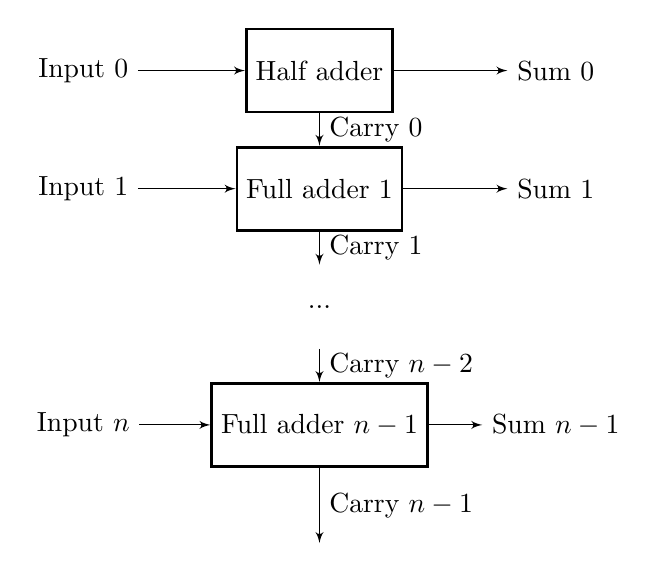
\begin{tikzpicture}[node distance=1.5cm]
            \node[block] (half) {Half adder};
            \node[block, below of=half] (full1) {Full adder 1};
            \node[empty, below of=full1] (dot) {...};
            \node[block, below of=dot] (fulln) {Full adder $n-1$};

            \node[empty, left of=half] (spacingl) {};
            \node[empty, right of=half] (spacingr) {};

            \node[empty, left of=spacingl] (in0) {Input 0};
            \node[empty, below of=in0] (in1) {Input 1};
            \node[empty, below of=in1] (vertspacel) {};
            \node[empty, below of=vertspacel] (inn) {Input $n$};

            \node[empty, right of=spacingr] (out0) {Sum 0};
            \node[empty, below of=out0] (out1) {Sum 1};
            \node[empty, below of=out1] (vertspacer) {};
            \node[empty, below of=vertspacer] (outn) {Sum $n-1$};
            \coordinate[below of=fulln] (carry);

            \path[draw, ->] (in0) -- (half);
            \path[draw, ->] (in1) -- (full1);
            \path[draw, ->] (inn) -- (fulln);

            \path[draw, ->] (half) -- (out0);
            \path[draw, ->] (full1) -- (out1);
            \path[draw, ->] (fulln) -- (outn);

            \path[draw, ->] (half) -- node [midway, right] {Carry 0} (full1);
            \path[draw, ->] (full1) -- node [midway, right] {Carry 1} (dot);
            \path[draw, ->] (dot) -- node [midway, right] {Carry $n-2$} (fulln);
            \path[draw, ->] (fulln) -- node [midway, right] {Carry $n-1$} (carry);
        \end{tikzpicture}
        \label{fig:n-bit-adder}
    \end{figure}
\end{frame}

\subsection{Implementation and testing}
\begin{frame}
    To implement this, we start by combining each of the sub circuits by using
    our basic logic gates, and by combining them into an $n$-bit adder.

    \vspace{\baselineskip}
    Then we test our circuit in the same manner as before, with a tester
    process.
\end{frame}


% exit section
\AtBeginSection{}
\section*{}

% {{{ Bibliography ------------------------------------------------------------
%\begin{frame}{Bibliography}
%  \tiny
%  \bibliographystyle{plain}
%  \bibliography{pl}
%\end{frame}
% }}} -------------------------------------------------------------------------

\end{document}
